\subsection {Verhalten Photovoltaik mit und ohne Energiespeicher}   % 2.5
    \subsubsection{Messung}                                             % 2.5 a
        \textbf{Methode}
        \newline
        \par Die Messungen werden wie in der Schaltskizze ausgeführt. Beim zweiten Durchlauf wird ein Kondensator parallelgeschaltet. Mit folgendem Matlab-Skript wurde Abbildung ~\ref{fig:matlab_langzeit_kondensator} dargestellt:
        
        \begin{figure}[h]
            \lstinputlisting[style=Matlab, firstline=19, lastline=24]{messungen/Aufgabe_2_5/import_data.m}
            \caption{Matlab-Skript zur grpahischen Darstellung der Spannung}
            \label{fig:matlab_langzeit_kondensator}
        \end{figure}

        
        \begin{figure}[H]
            %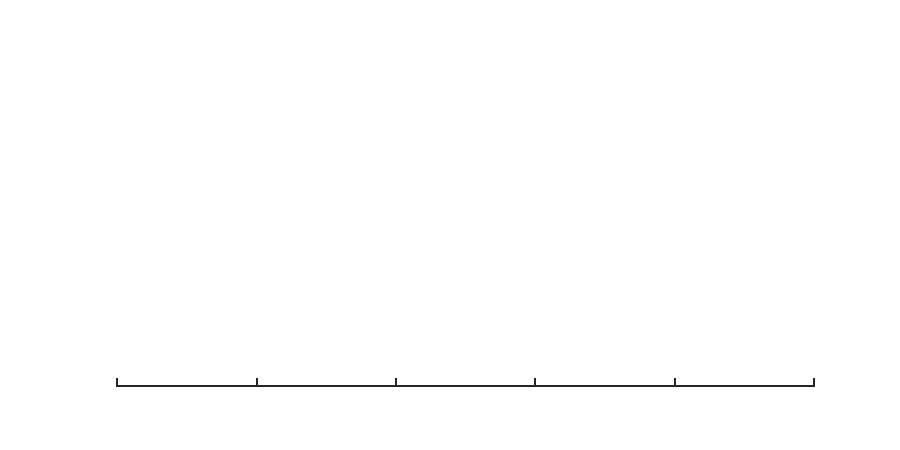
\includegraphics{spannung_kondensator}
            \def\svgwidth{\textwidth}
            \input{spannung_kondensator.pdf_tex}   
            %\centering
            %\def\svgwidth{\columnwidth}
            %\input{.pdf_tex}
            \caption{Spannungsverlauf mit und ohne Kondensator}
    \end{figure}
        
    \subsubsection{Auswirkung des Speicherkondensators}                 % 2.5 b
        \textbf{Diskussion}
        \newline
        \par Auf dem ersten Blick fallen die Werte der Messung ohne dem Kondensator auf, welche trotz gleichmäßiger Beleuchtung um einen Mittelwert, einer Spannungskonstante, schwanken. Solche oszillierende(?) Werte treten mit einem Kondensator nicht auf. Schaltet man einen Kondensator dazu, so erreicht dieser erst nach ca. 10 Minuten Beleuchtung die Spannungskonstante der Schaltung ohne Kondensator. Der Graph steigt exponentiell an, sodass mit der Zeit die Spannungsänderung kleiner wird. Wird die Solarzelle im Anschluss beschattet, so fällt der Graph im Gegensatz zu der ohne dem Kondensator exponentiell, weshalb die Spannung in der kurzen Beschattungszeit auf ungefähr 0,5V statt auf 0V sinkt. Der Übergang zwischen den beiden Phasen bei dem Graphen ohne dem Kondensator hingegen ist abrupt.
        \par Betrachtet man die Werte im Intervall, in der alle 30 Sekunden die Phase wechselt, so lässt sich feststellen, dass bei der ersten Messung die Spannung bei jeder Bestrahlung näherungsweise gleich hoch ist. Bei der zweiten jedoch nimmt die maximale Spannung mit jedem Durchlauf ab. 
        \par Allgemein lässt sich sagen, dass ohne einem Kondensator bei konstantem Lichteinfall die Spannung gleichbleibt und bei der Verschattungszeit diese auf null fällt. Der Wechsel zwischen den beiden Phasen verläuft annähernd sprunghaft. Mit einem Kondensator steigt die Spannung exponentiell an unter Lichteinfluss. Bei Abwesenheit dieser nimmt die Spannung dementsprechend exponentiell ab.
        
        %\par Speicherkondensatoren können daher auch als Energiespeicher fungieren, jedoch sind diese nur teils dafür geeignet. Während der Entladung nimmt die Spannung mit der Zeit ab, sodass sie nicht als konstante Spannungsquelle infrage kommt. Nichtsdestotrotz ist von Vorteil, dass der Kondensator die elektrische Energie direkt speichert, ohne diese in eine andere Energie umzuwandeln.
        
        
        
        
        \par (zu überarbeiten: Speicherkondensatoren können daher als Energiespeicher fungieren, jedoch sind diese nur teils dafür geeignet. Während der Entladung nimmt die Spannung mit der Zeit ab, sodass sie sich nicht als konstante Spannungsquelle infrage kommt.
        Nichtsdestotrotz ist von Vorteil, dass der Kondensator die elektrische Energie direkt speichert, ohne diese in eine andere Energie umzuwandeln.)

        
        
        
        \par Bei erneuerbarer Energie sind die schwankenden Umweltfaktoren entscheidend. So wurde zuvor (vgl. 2.3) abgeschätzt, wie stark sich die Messung in der Sommerzeit verändert hätte. Bei einer Solarzelle kommen noch weitere Einflüsse wie Verschattung und Einfallswinkel des Lichts hinzu. In diesen Momenten wirkt der Speicherkondensator einem direkten Abbruch der Spannung entgegen. Daher spielt bei den erneuerbaren Energien die Energiespeicherung eine besonders große Rolle. Zwar helfen Speicherkondensatoren bei kürzeren Spannungseinbrüchen, jedoch stellt sich eine langanhaltende Speicherung als schwierig heraus, da der Speicher selber in Laufe der Zeit Energie verliert (Quelle), sodass es wirtschaftlich effizienter ist, die Energie in einer anderen Energieart zwischen zu speichern trotz Energieverlust bei den Umwandlungen. (Quelle) 


